\section{Object Partition}
\label{sec:surf_part}

\ichao{\figname~\ref{fig:nearest} and \figname~\ref{fig:cut_plane}} can be merged into one.

As mentioned \chireplace{in}{at} the beginning of this paper, most of the consumer-level 3D printers have limited printing volumes.
In order to print our large-scale object, it is necessary to decompose the object into different partitions.
Meanwhile, unlike traditional surface partition methods that only take surface features into consideration, we also need to consider the relationship between the outer surface partitions and the inner optimized Zometool structure.
More specifically, we will place connectors between the outer and inner structure in order to connect them (we will describe the design of the connector in more detail in~\secname~\ref{}).
% We aim to decompose the surface into different partitions for 3D printing
% with the optimized Zometool structure $\mathbf{Z}$ from \secname~\ref{sec:Zometool}.
Naively, we can simply compute the distance from each triangle $t$ to all the nodes in $\mathbf{Z}$, and assign $t$ to the nearest node as it's label.
However, inconsistency may arise among adjacent triangles, leading to unsatisfactory visual effects and assembly complexities (numerous small partitions might exist, see \figname~\ref{fig:nearest}). 
To address this issue, we formulate the problem as a multi-label graph cut minimization.
As each triangle $t$ can potentially correspond to different Zometool node\chinky{s}, it gets assigned data cost for different corresponding nodes.
Given $n$ elements, $k$ labels and $n\cdot k$ costs, finding the minimum assignment is a combinatorial problem and typical NP-hard.
We employ Boykov~\cite{boykov:2004:experimental} to solve it.

After the partition, we further regularize the boundaries between pieces by performing a multi-class classification.
The \chireplace{major}{} reason is that we seek smooth boundaries in order to ease the assembling process.
% we have to find the method which can separate different labels. 
% There are many partition methods we can choose. Because our result have to assemble, our segment can't have the sharp edges which may increase the assembling complexity. The planar-cut is our first choice. 
We follow Wang~\cite{wang2016improved} and use the Support Vector Machine (SVM)~\cite{cortes1995support} classifier to find our cut-plane. 
We will describe the detail formulation and implementation of MRF problem and how to find the cut planes in the following paragraph.
% The following context will describe more implementation details about graph cut and cut-plane.

\begin{figure}[ht]
\centering
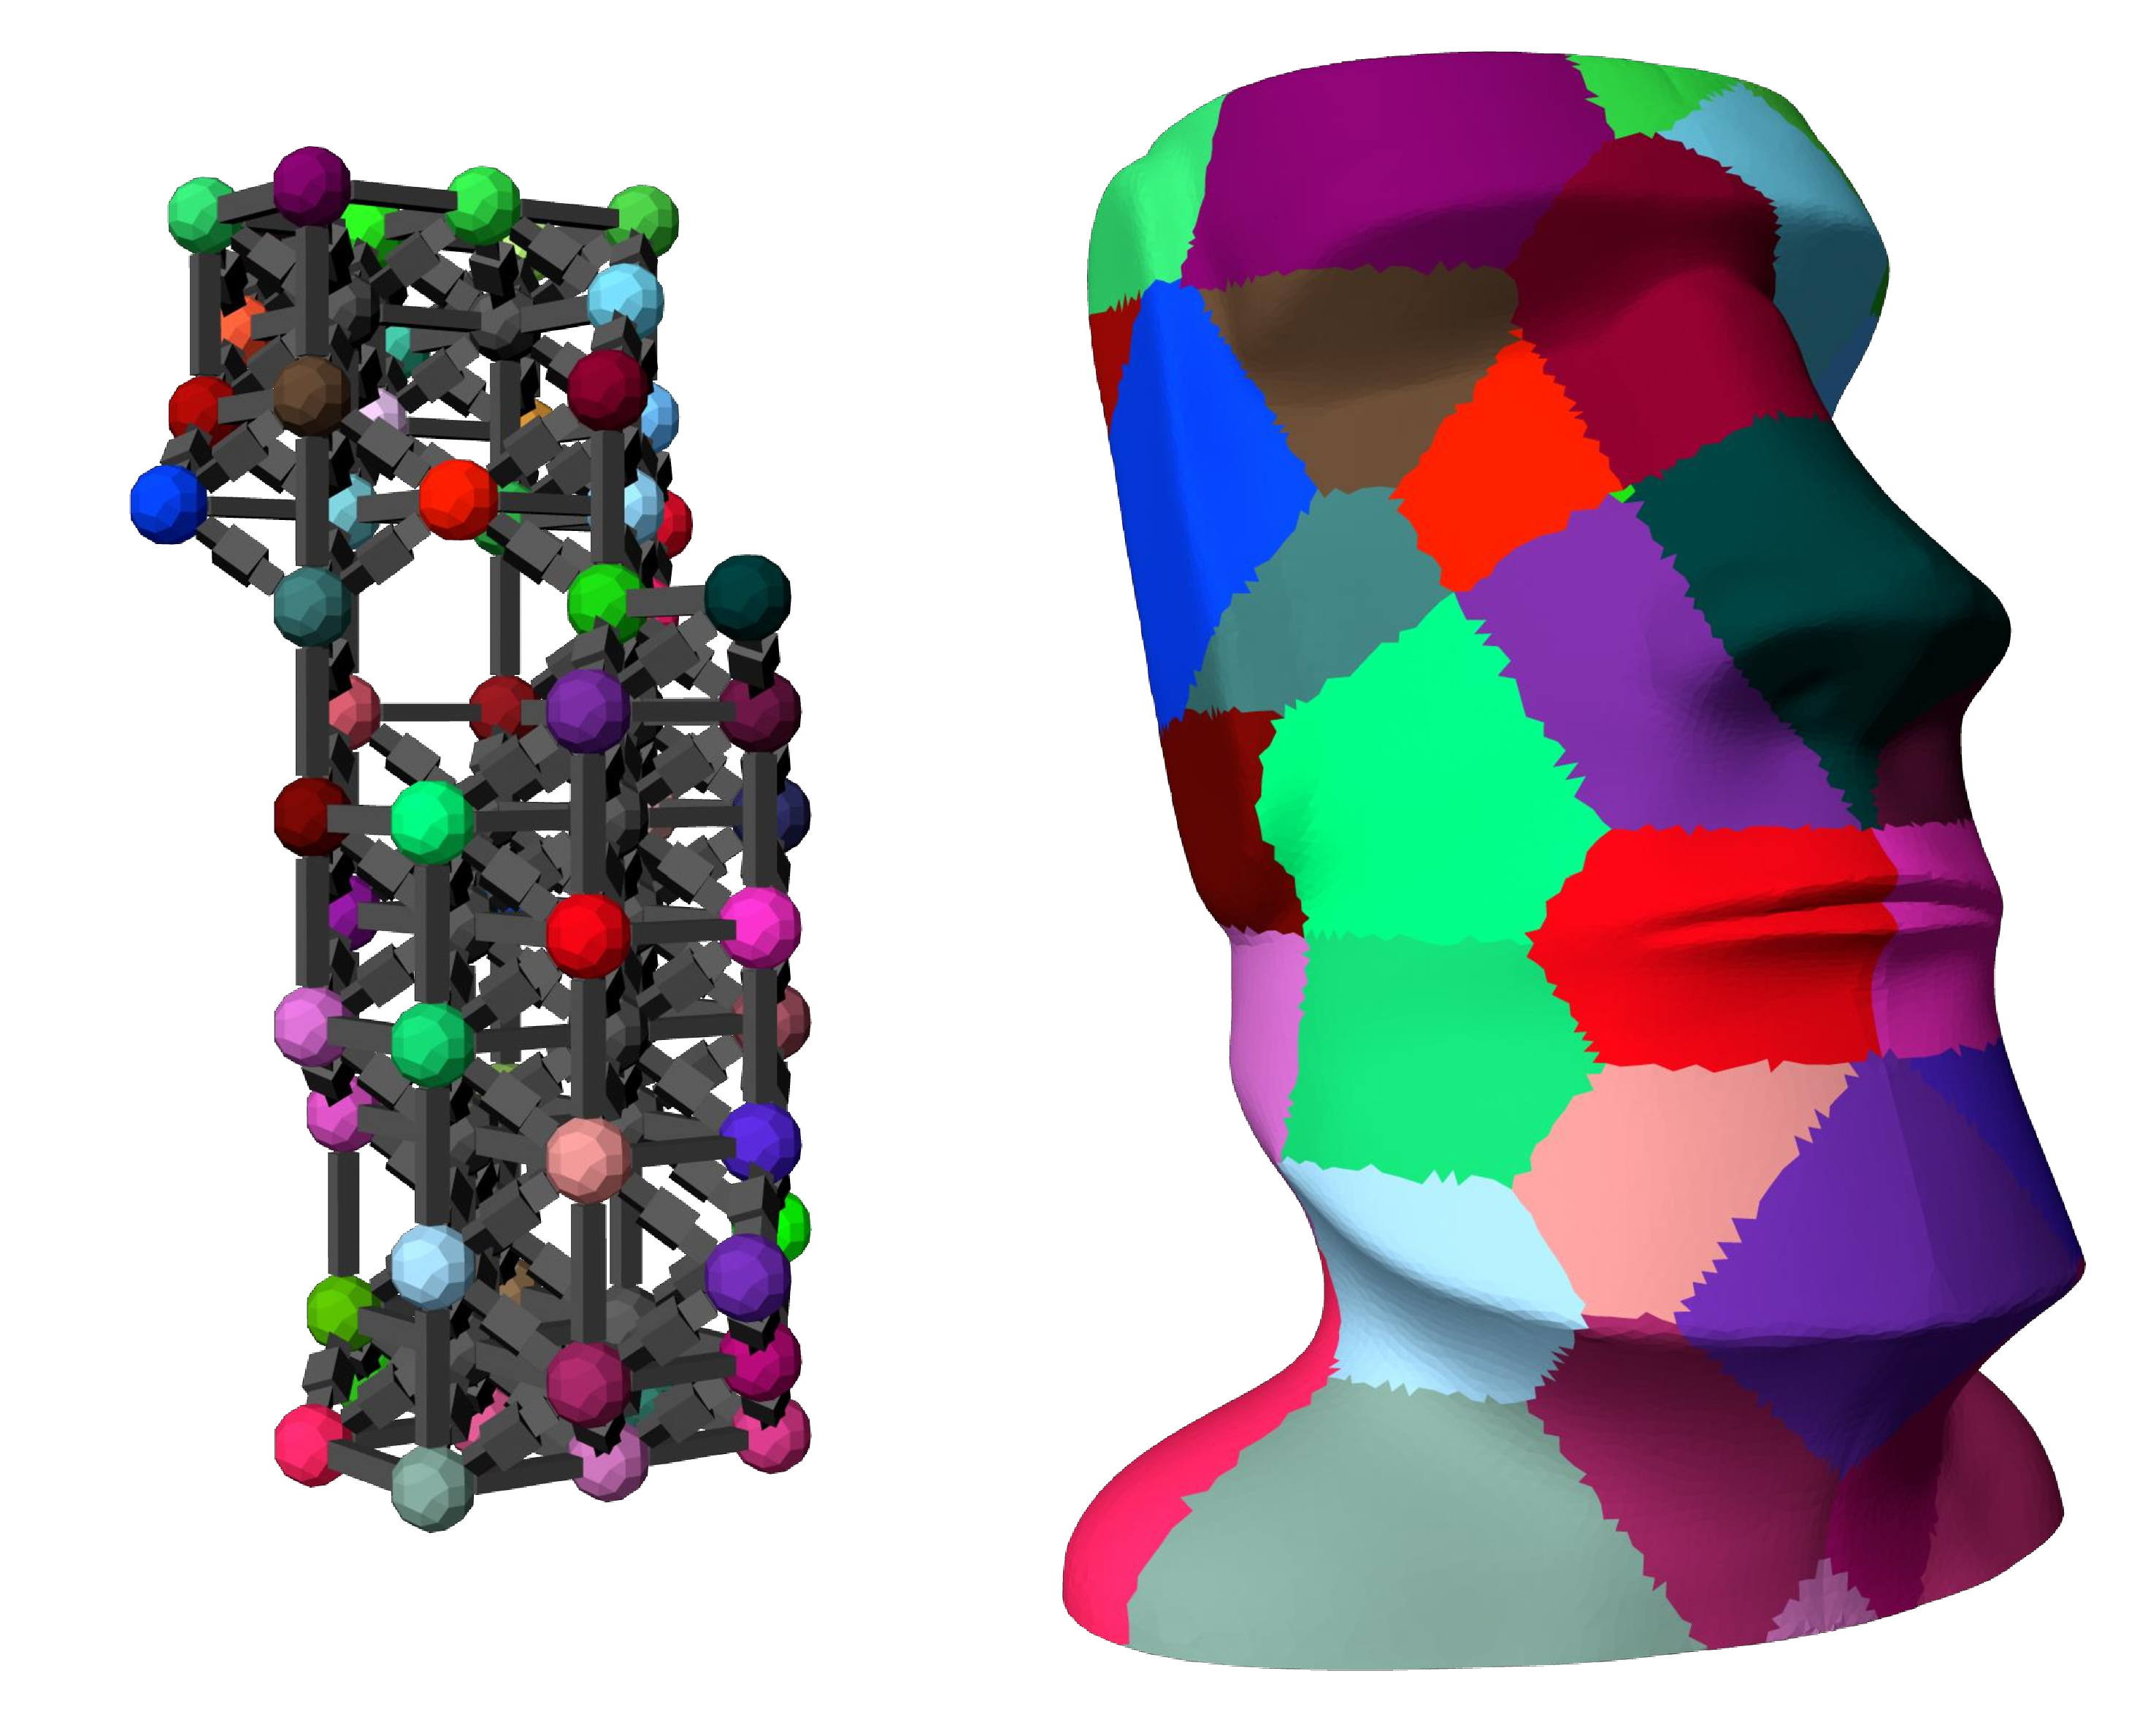
\includegraphics[width=0.75\linewidth]{figs/nearest_node.pdf} 
\caption{Simple classification. We assign each triangle to it's nearest node. But there are too many labels and some regions are too small for 3D printer to print it, So, we need to reclassify the result.}
\label{fig:nearest}
\end{figure}

\subsection{Surface Partition}
\paragraph{Optimization energy}
We compute the assignment function $f$ that assign label\chinky{s} to each triangle $t$, where $t \in T$, such that the labeling $f$ minimize the following energy $E(f)$:
\begin{align} \label{eq:graph}
E(f) = w_{data} * \sum_{t\in T}D(t, f_t) + w_{smoothness} * \sum_{t,s\in N} S(t, s, f_t, f_s),
\end{align}
and we optimize this function using multi-label graph-cut algorithm proposed by Boykov~\cite{boykov:2004:experimental}.
In our setting, the entire outer nodes of $\mathcal{Z}$ are complete possible label set $L$.
This $E(f)$ consists of two separate terms, i.e.\chinky{,} data and smoothness.
Next, we will explain each term in more detail.

\subsubsection{Data cost}
Data cost measures how well a triangle $t$ covers a node $p \in P$.
This cost is simply defined as the distance of the nearest node to the triangle.
\begin{align}
D(t, f_t) = -\omega \log(\mathcal{P}(p | t)),
% D(p,f_p) = \displaystyle\min_{p \in P}(d(t, p))
\end{align}
where $\mathcal{P}(p | t)$ is the probability of that triangle $t$ belong to the node label $p$, and $\omega$ is a constant that
regulates the influence of the data term in the total energy.
Here, we simply define $\mathcal{P}(p | t)$ as $1/d(t,p)$, where $d(t,p)$ is the distance of the node to the triangle.
\subsubsection{Smoothness cost}
Smoothness term measures the spatial consistency of neighboring elements.
\begin{align}
S(t, s, l_t, l_s) = 
\begin{cases}
0, & \text{if } l_t = l_s, \\
-\log(\theta_{t,s}/\pi)\varphi_{t,s} + w_{saliency} * E_{saliency}(t), & \text{otherwise} 
\end{cases}
\end{align}
where $\theta_{p,q}$ and $\varphi_{p,q}$ are the dihedral angle and distance between triangle $p$ and $q$, respectively.
With the smoothness term, two adjacent triangles are likely to have consistent labels.

\paragraph{User-guided saliency} 
We observed that there are many salient regions on each of the object we used, e.g., we don't want the partition seam to go through the eyes and nose on the face \chireplace{~\figname~\ref{fig:saliency}}{(see ~\figname~\ref{fig:saliency})}.
\chireplace{In order to}{To} preserve the salient region, we ask users to draw the region he thinks it's important to preserve, and we formulate this as part of the smoothness cost, which prevent\chinky{s} \chireplace{the partition seam}{partition seams} to cut through salient region\chireplace{~\figname~\ref{fig:saliency}}{(~\figname~\ref{fig:saliency})}..
% Every mesh have some features, such as eyes, nose or other unique objects. 
% But we can't get the feature information by only use relation of adjacent triangles. 
% If we don't assign some information during process of graph cut, the result just like left of \figname~\ref{fig:saliency}, the mouth and nose will be split in later process. Our saliency information is given by user guidance. For example (see middle of \figname~\ref{fig:saliency}), the user think the mouse and the nose is the important feature on mesh, so mark those parts and hope the parts don't be split in later process. Since we give the saliency information, the marked regions usually assign in the same part and prevent the slice seam on those regions.

\begin{align}
E_{saliency}(t) = 
\begin{cases}
1, & \text{triangle is marked as salient region}, \\
0, & \text{otherwise} 
\end{cases}
\end{align}

\begin{figure}[ht]
\centering
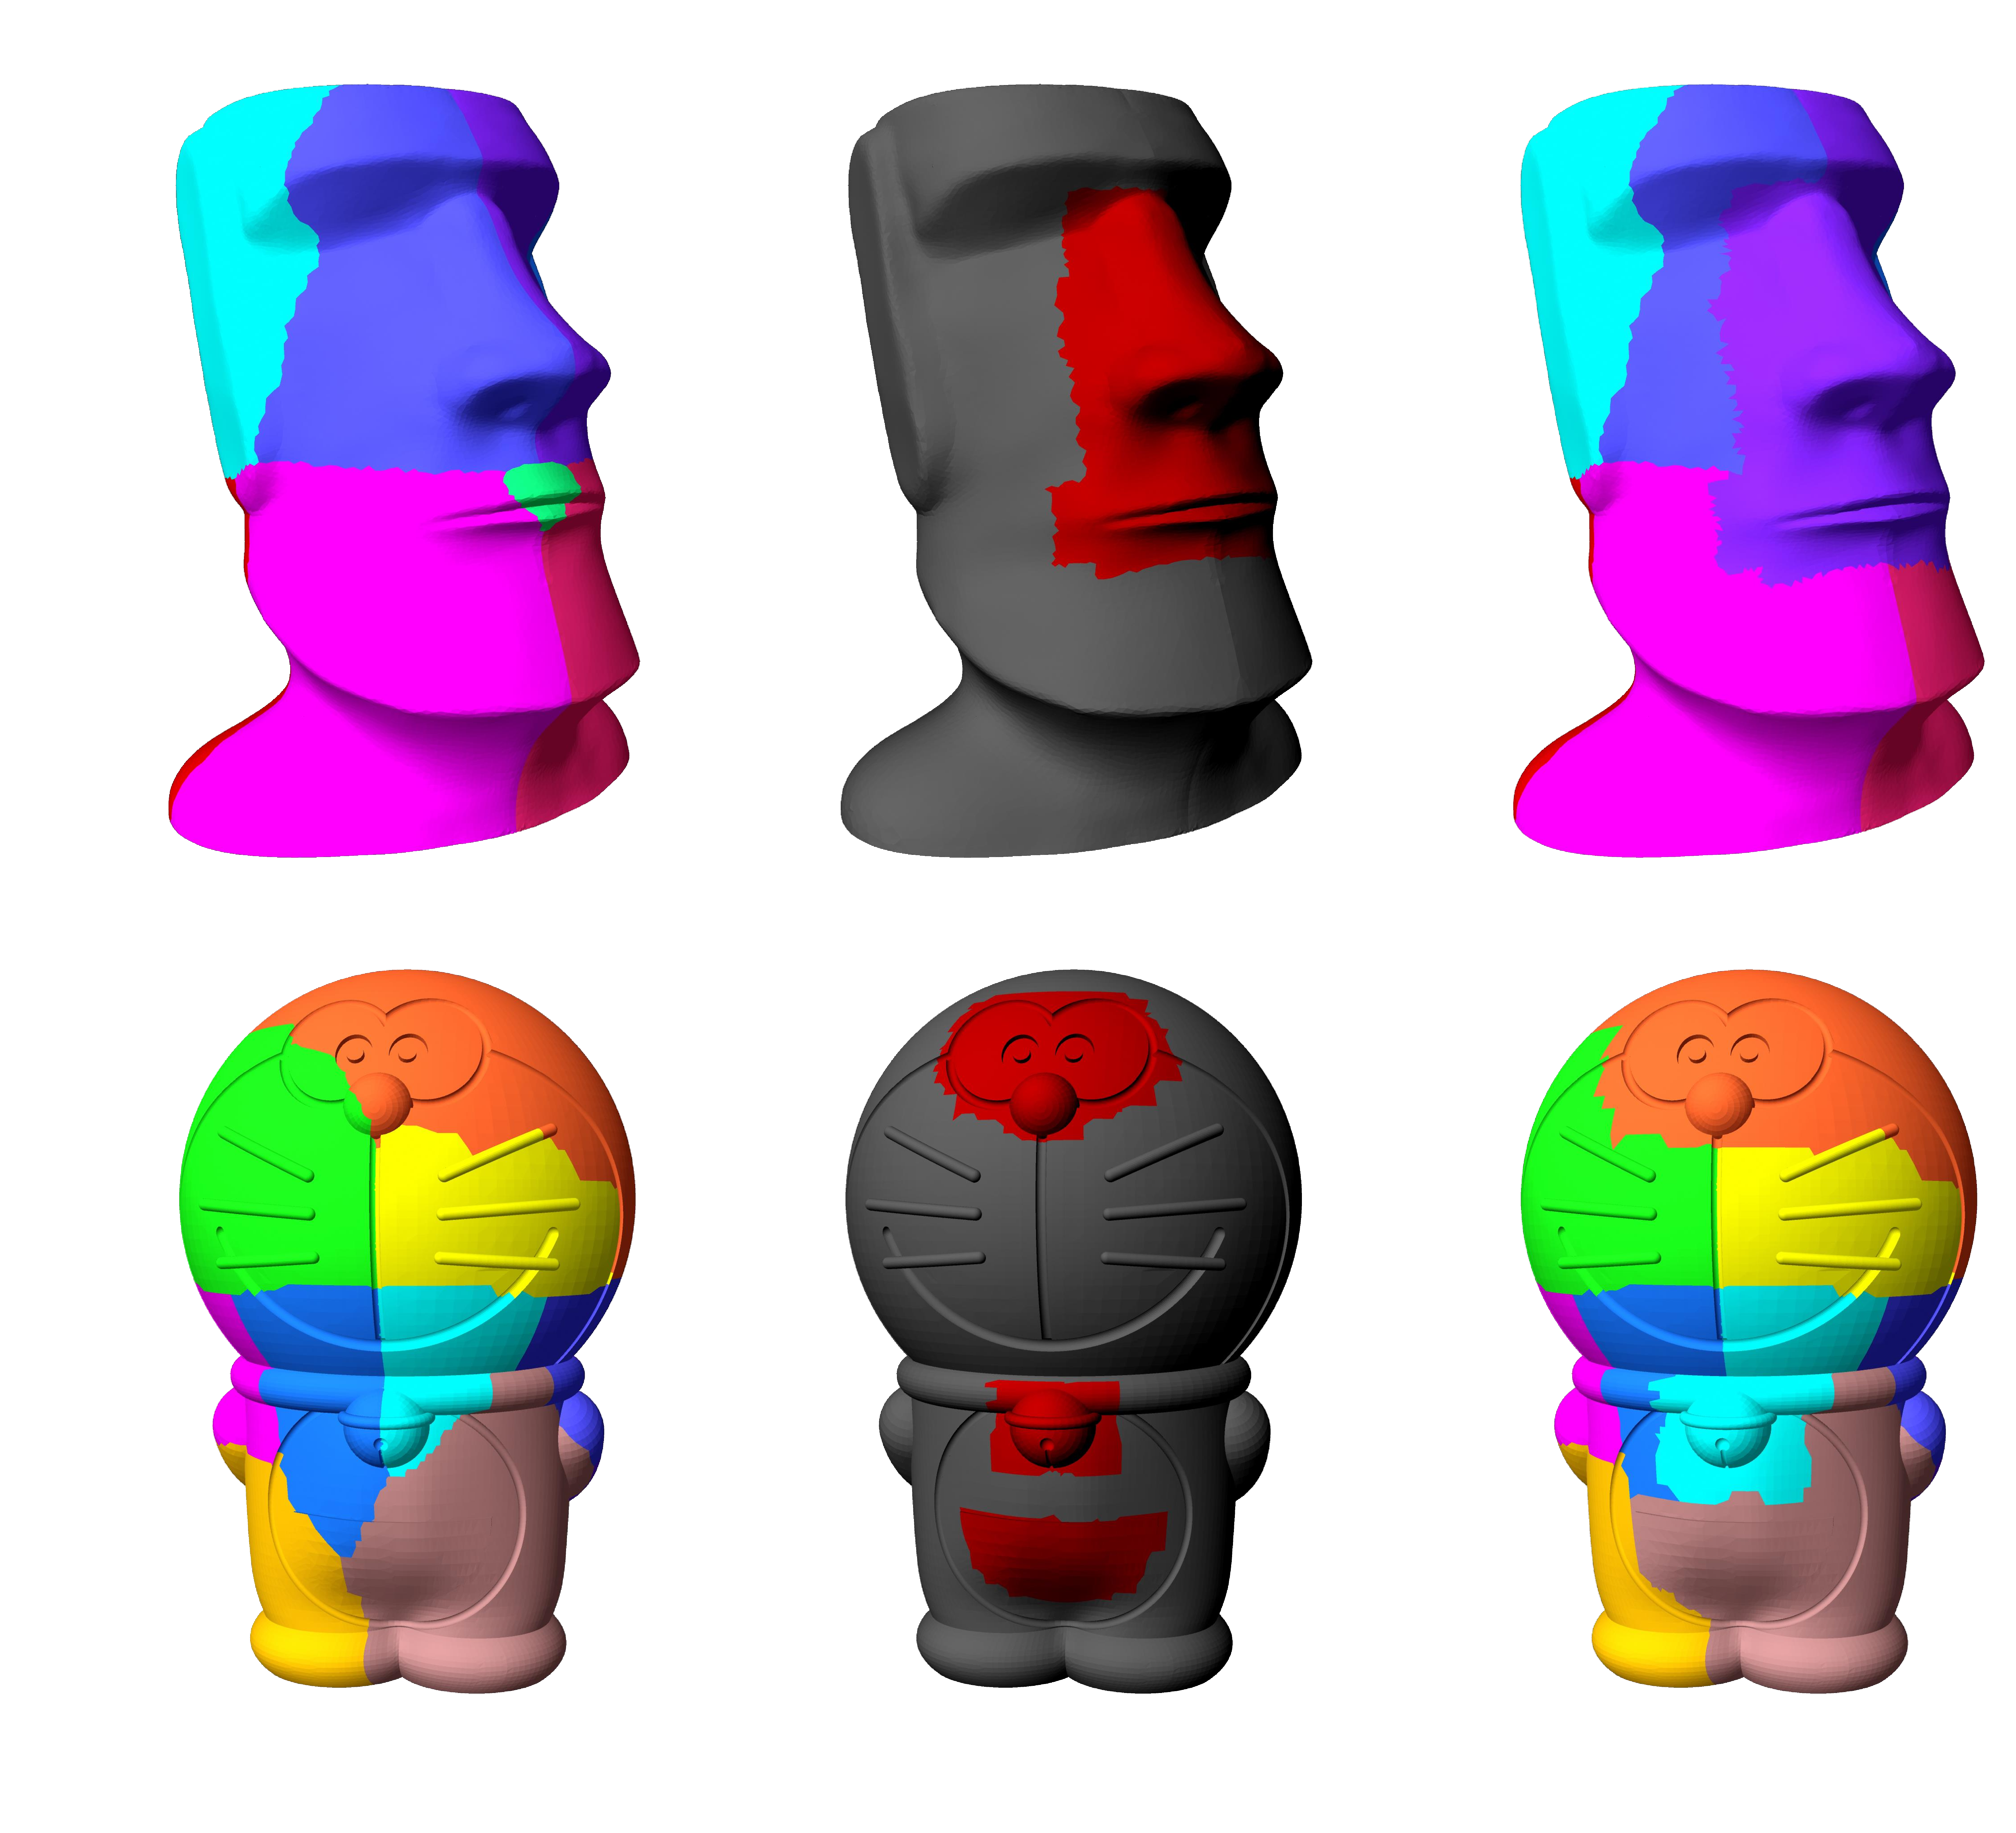
\includegraphics[width=1.0\linewidth]{figs/saliency.pdf} 
\caption{User-guided saliency. 
Origin result of graph cut may split some feature on the mesh. (Left of the figure) In order to solve it, we ask user to mark the unique feature. (Red region in the middle of the figure) We add those information for graph cut, and precent those regions from separating into multiple parts. (Right of the figure)} 
\label{fig:saliency}
\end{figure}

\subsubsection{Our result}
We solve the labeling problem~\eqname~\ref{eq:graph} with graph-cut and obtain 11 labels on the Maoi head object~\figname~\ref{fig:cut_plane}(a).
Compare to the naive method (\figname~\ref{fig:nearest}), we obtain \chinky{much} smaller partition numbers (11 v.s. 60), and each of them \chireplace{are}{is} with better shape and size.
% Each label has better shape and size than that before reclassification. (See \figname~\ref{fig:cut_plane}(a)) Then, we have to separate each label into pieces for 3{D} printing.
% Before the labeling optimization, there are too many labels (60 labels in \figname~\ref{fig:nearest}) and some labels are too small. 
% By optimizing~\eqname~\ref{eq:mrf},
% Therefore, we use graph cut algorithm to optimize the energy function (Equation \ref{eq:graph}) which we design the data and smoothness cost. After the optimization, we get the result which has 11 labels. Each label has better shape and size than that before reclassification. (See \figname~\ref{fig:cut_plane}(a)) Then, we have to separate each label into pieces for 3{D} printing.

\subsection{Object Cut}
% There are many methods for mesh segmentation. The simple method is collecting all triangles of graph cut label, but it will cause the sharp edge. 
In order to cut the physical object into pieces, we have to find the cut planes that separate the space occupied by the object.
However, the boundaries between optimized partitions from \chinky{the} previous step \chireplace{is}{are} not regularized enough for directly used as the separating plane. 
% For easy assembling, we have to split the triangles and regularize the contact surface between different labels. 
% We choose the planar cut for our method.
It is very difficult to find a plane in 3{D} space because of the varied plane normal vectors.
\chireplace{In order to}{To} obtain the desired cut planes, we analogize our problem to finding the separating plane in solving multi-class classification using Support Vector Machine (SVM).
We use each triangle as a data sample, with it's location as \chinky{the} feature vector and the optimized label from \chinky{the} previous step as it's class.
In short, SVM algorithm intend to find the best hyperplane which is the one that represents the largest separation, or margin, between the two adjacent classes. 
\chireplace{And}{Therefore,} we use the obtained hyperplanes from SVM as our cut planes (\figname~\ref{fig:cut_plane}(b)).

% We use the SVM classifier to generate the cut-plane. The different label of vertex is our input for training. Then, we can get the hyperplane which will separate different labels of data. But we don't have to know the hyperplane which separate the nonadjacent labels. So before we start training, we find the neighbor pair and use the information that can let us know which hyperplane needs for split the label.  By collecting all the hyperplanes, like \figname~\ref{fig:cut_plane}, we can use those planes for segmentation.

\begin{figure}[ht]
\centering
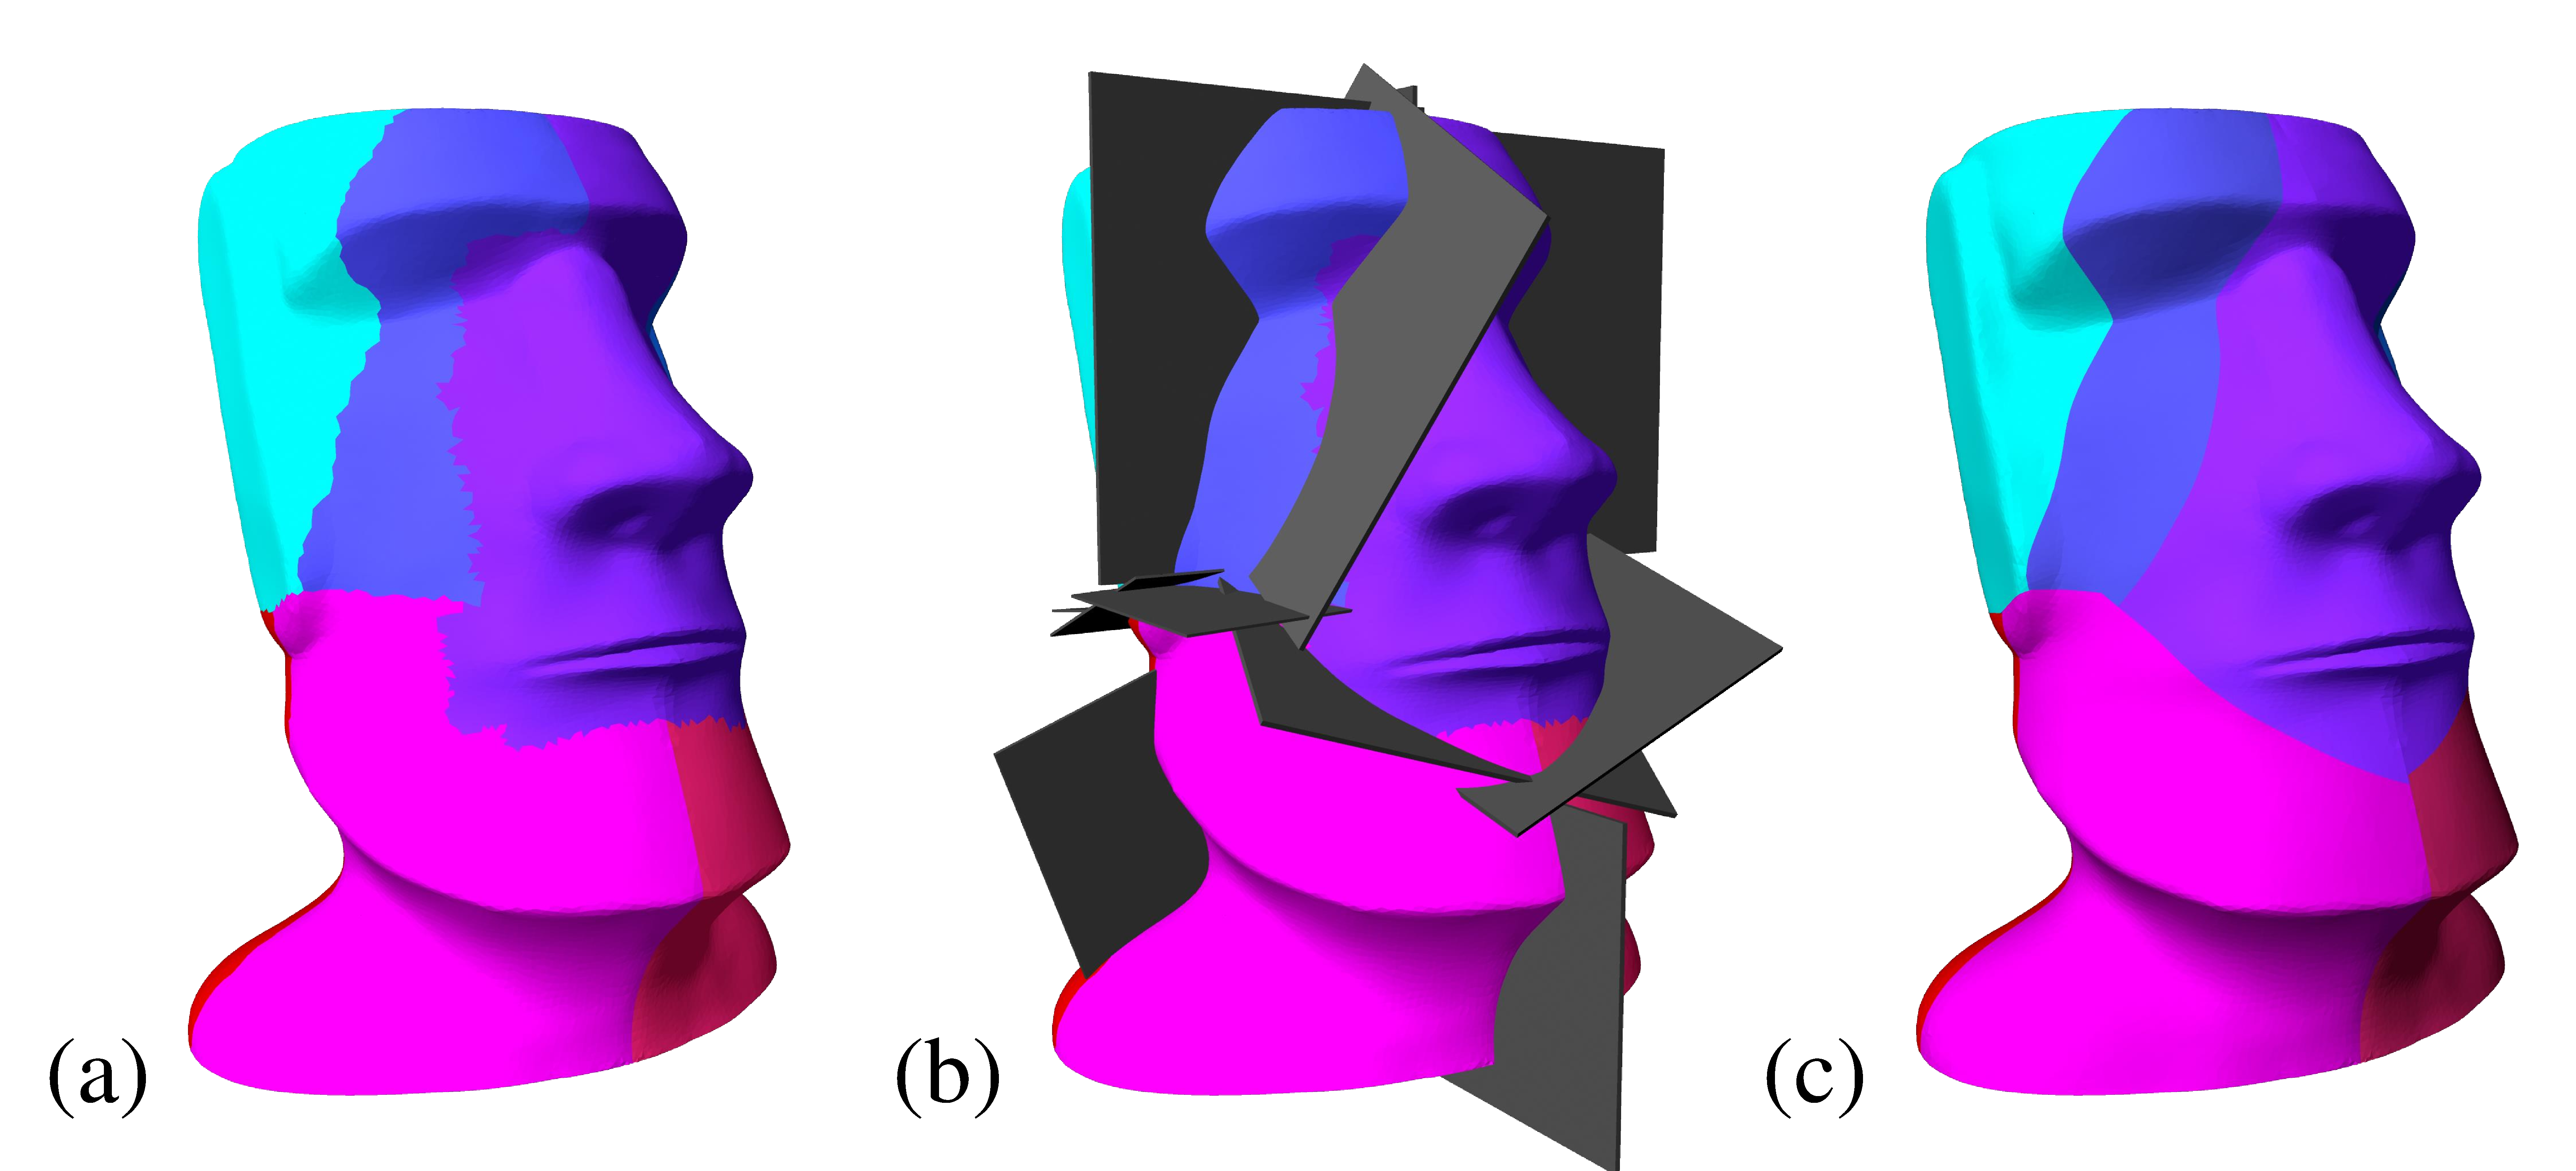
\includegraphics[width=1.0\linewidth]{figs/cut_plane1.pdf} 
\caption{(a) Result of graph cut (b) Cut-plane generated by SVM classifier (c) Cutting result} 
\label{fig:cut_plane}
\end{figure}

